% testing.tex

\chapter{Testing and debugging the application}
\label{chap:testing}
Testing and debugging applications under development is usually not very
difficult. As soon as the application starts to work with events like signals
and slots debugging can become difficult.

\bigskip \noindent
The main goal of this chapter is to present the testing and debugging methods
used, in particular the way Qt's signal/slot mechanism was debugged.

\bigskip \noindent
Section \ref{chap:testing:cycle} discusses the general test -- debug -- develop
cycle commonly used by the programmer. Section \ref{chap:testing:techniques}
will focus more on the debugging techniques applicable to signal/slot
debugging.

\section{The test -- debug -- develop cycle} \label{chap:testing:cycle}
The general test -- debug -- develop cycle is depicted in Figure
\ref{fig:testing:cycle}. The diagram starts with the applications' source code
at some point in time. This source must be compiled to obtain the executable.
If a typing error was made or a method forgotten to implement, the compiler or
linker will not be successful and the source must be edited. This is usually
due to a simple mistake on the programmers part.

\bigskip \noindent
After the source code has been successfully compiled and linked, the
functionality just added to application needs to be tested. This is represented
by the input of test vectors. What these test vectors are, depends on the
application and the functionality being tested. The tester (in this case the
programmer) then either marks the added functionality as successful or
unsuccessful.

If testing was successful, the programmer can continue to implement the next
feature. If testing failed, a bug is present in the application. The bug must
then be located. The bug is usually related to feature that was added but this
is not necessarily the case (either because of poor testing or because some
other part of the code could not be tested before this part was ready).

\bigskip \noindent
Locating a true bug can be quite difficult. It is usually the most
time-consuming part of development and is therefore shown in grey in the
figure. Once the bug has been identified a solution can be found easily in most
cases. The cycle then continues normally.

\begin{figure} \begin{center}
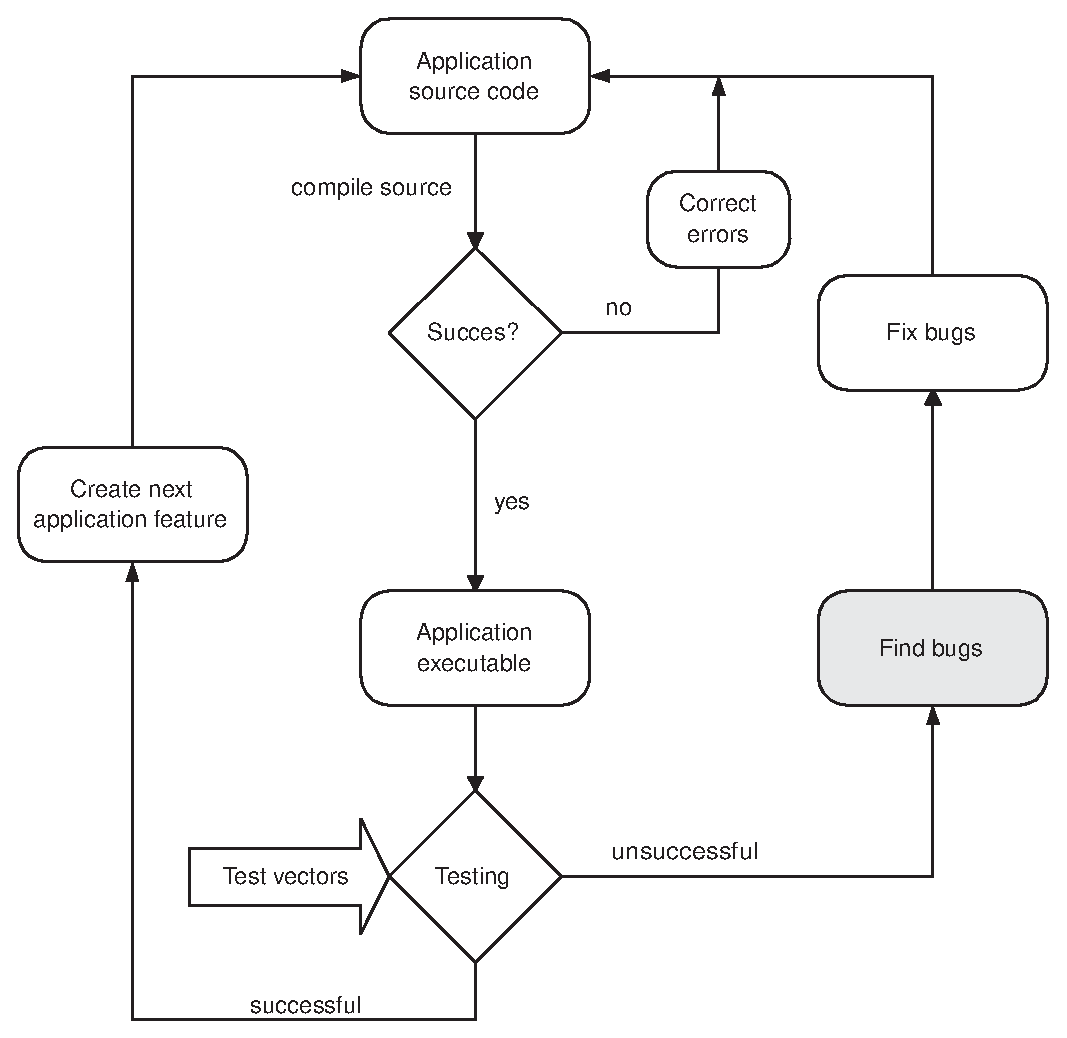
\includegraphics[width=10cm]{./figures/testcycle.eps}
\caption{The test -- debug -- develop cycle}
\label{fig:testing:cycle}
\end{center} \end{figure}

%%% Nick seemed to like this very much (001208)
\section{Debug techniques used} \label{chap:testing:techniques}
The best technique to find a bug depends on the type of bug encountered. The
bugs encountered most are:
\begin{itemize}
\item Unexpected behaviour. The application does not perform its task correctly
or not all.
\item Segmentation faults/bus errors. The application ``crashes''. Segmentation faults are usually due to
an abused pointer.
\item Crashes or unexpected behaviour associated with signals/slots.
\end{itemize}
Useful approaches for finding the location (or reason) for these bugs will be
discussed next.

\subsection{Unexpected behaviour}
An example of unexpected behaviour could be the erroneous generation of the
text resulting from the \verb=foreach= loops in the configuration file. The
algorithm was either not correct or not correctly implemented. To ascertain the
exact location or reason for this bug it necessary to gain more insight into
how the algorithm is ``run''.

The best way to gain insight into the inner workings of an algorithm is by
using a debugger. An excellent debugger is \verb=gdb=. Unfortunately, it has no
graphical front end. This means some experience is required to use \verb=gdb=
effectively. It is therefore recommended to use a graphical front-end to
\verb=gdb= like \verb=DDD= (the Data Display Debugger), \verb=xgdb= or even \verb=xemacs=.
Another option is \verb=kdbg=. These debuggers allow step-by-step execution of
the source code and inspection of the values of the variables used.


\bigskip \noindent
Another useful method could be to use debug statements. These print out
information about the state of the application at strategic places. If a smart
\verb=#define= statement is used it is possible to disable the output for
release builds.

\subsection{Locating segmentation faults}
Contrary to unexpected behaviour, segmentation faults can be located quite
easily. If the application is run from the debugger it will report the location
the segmentation fault occurred. In \verb=gdb= this can be done with the
backtrace command \verb=bt=. This lists a backtrace of the stack, showing
exactly how the application reached the point where the segmentation fault
occurred.

Once the location of the segmentation fault is known the reason for it is
usually (but not always) clear and fixing the bug can begin.

\subsection{Signal/slot debugging}
The signal/slot mechanism provided by Qt presents a challenge in case of bugs.
Segmentation faults that occur right after a signal can be extremely difficult
to locate or solve.

The signal/slot mechanism is available to any class that inherits the
\verb=QObject= class. This includes all widgets. If a backtrace of the stack is
requested right after a segmentation fault it will only display methods used by
these Qt objects. It is very difficult to pinpoint the exact object that sent
the signal (and often caused the error).

\paragraph{A common signal/slot pitfall\\ }
An error often made that is difficult to find is the deletion of the sending
object from the receiving slot. For example, object \verb=A= sends a signal to
object \verb=B=. Because of this signal, \verb=B= tells the manager of \verb=A=
objects \verb=C= to delete certain \verb=A= objects. If one of these \verb=A=
objects was the object that originally sent the message a segmentation fault is
very likely.

The reason for this is the fact that emitting a signal is nothing more than
calling a method. Once the signal method completes it will eventually return to
the place the signal was emitted. If that object has been deleted this location
is no longer valid and a segmentation fault will occur.

For more insights into how the signal/slot mechanism is implemented the
interested user is recommend to take a look at the output of the
\verb=meta object compiler= and the source of the \verb=QObject= class.

\bigskip \noindent
\paragraph{Tips\\}
Some additional tips:
\begin{itemize}
\item Compile Qt with debugging on and use this library during development.
Warnings about unconnected signals/slots will then be issued by Qt. It is also
possible to dump information about a \verb=QObject= tree.
\item The meta object compiler \verb=moc= also has a debugging feature.
Enabling this feature can be useful to track signals/slots.
\end{itemize}
